\documentclass[a4paper]{article}
\usepackage{algorithm}
\usepackage{algorithmicx}
\usepackage{algpseudocode}
\usepackage{graphicx}
\usepackage{epstopdf}
\usepackage{placeins}
\usepackage{amsmath}
\usepackage{array}
\usepackage{ctex}
\usepackage{geometry}
\usepackage{mdwlist}
\usepackage{amsbsy}
\usepackage{amssymb}
\usepackage{enumitem}
\usepackage{tikz}
\usepackage{xcolor}
\usepackage{listings}
\usepackage{multirow}
\usepackage{booktabs}
\usepackage{float}
\usepackage{framed}
\usepackage{color}
\definecolor{lightgray}{rgb}{0.75,0.75,0.75}
\newenvironment{lightgrayleftbar}{%
  \def\FrameCommand{\textcolor{lightgray}{\vrule width 3pt} \hspace{3pt}}%
  \MakeFramed {\advance\hsize-\width \FrameRestore}}%
{\endMakeFramed}
\usetikzlibrary{trees}
\geometry{a4paper,scale=0.75}
\setlist[description]{leftmargin=*}
% \setmainfont{Times New Roman}
\lstdefinestyle{lfonts}{
    basicstyle   = \footnotesize\ttfamily,
    stringstyle  = \color{purple},
    keywordstyle = \color{blue!60!black}\bfseries,
    commentstyle = \color{olive}\scshape,
}
\lstdefinestyle{lnumbers}{
    numbers     = left,
    numberstyle = \tiny,
    numbersep   = 1em,
    firstnumber = 1,
    stepnumber  = 1,
}
\lstdefinestyle{llayout}{
    breaklines       = true,
    tabsize          = 2,
    columns          = flexible,
}
\lstdefinestyle{lgeometry}{
    xleftmargin      = 20pt,
    xrightmargin     = 0pt,
    frame            = tb,
    framesep         = \fboxsep,
    framexleftmargin = 20pt,
}
\lstdefinestyle{lgeneral}{
    style = lfonts,
    style = lnumbers,
    style = llayout,
    style = lgeometry,
}
\lstdefinestyle{python}{
    language = {Python},
    style    = lgeneral,
}

\renewcommand{\algorithmicrequire}{\textbf{Input:}}  % Use Input in the format of Algorithm
\renewcommand{\algorithmicensure}{\textbf{Output:}} % Use Output in the format of Algorithm

\makeatletter
\newenvironment{breakablealgorithm}
  {% \begin{breakablealgorithm}
   \begin{center}
     \refstepcounter{algorithm}% New algorithm
     \hrule height.8pt depth0pt \kern2pt% \@fs@pre for \@fs@ruled
     \renewcommand{\caption}[2][\relax]{% Make a new \caption
       {\raggedright\textbf{\ALG@name~\thealgorithm} ##2\par}%
       \ifx\relax##1\relax % #1 is \relax
         \addcontentsline{loa}{algorithm}{\protect\numberline{\thealgorithm}##2}%
       \else % #1 is not \relax
         \addcontentsline{loa}{algorithm}{\protect\numberline{\thealgorithm}##1}%
       \fi
       \kern2pt\hrule\kern2pt
     }
  }{% \end{breakablealgorithm}
     \kern2pt\hrule\relax% \@fs@post for \@fs@ruled
   \end{center}
  }

\renewcommand{\labelitemii}{$\circ$}
\makeatother

\title{人工智能导论------情感分析实验报告}
\author{计 93 王哲凡 2019011200}

\date{\today}

\begin{document}
    \maketitle
    \tableofcontents

    \newpage
    \section{模型分析}

    \subsection{模型抽象}
    每个评论的句子是由多个单词的组成的,假设一个句子有 $n$ 个单词,第 $i(1 \le i \le n)$ 个单词记为 $x_i$,我们可以利用 Word-Embedding 方法将其表示为 $k$ 维的向量,即 $x_i \in \mathbb{R}^k$。

    \begin{lightgrayleftbar}
        本实验中采用的词向量均为训练得出,未使用任何开源的预训练的词向量。
    \end{lightgrayleftbar}

    因此一个句子可以表示为:
    $$
    X_{1: n} = (x_1, x_2, \cdots, x_n)^T \in \mathbb{R}^{n \times k}
    $$

    实验中为了方便模型训练,统一通过 padding 方式将同一个 Batch 中的句子填充到相同的长度。

    \subsection{CNN 模型}

    \begin{figure}[h]
        \centering
        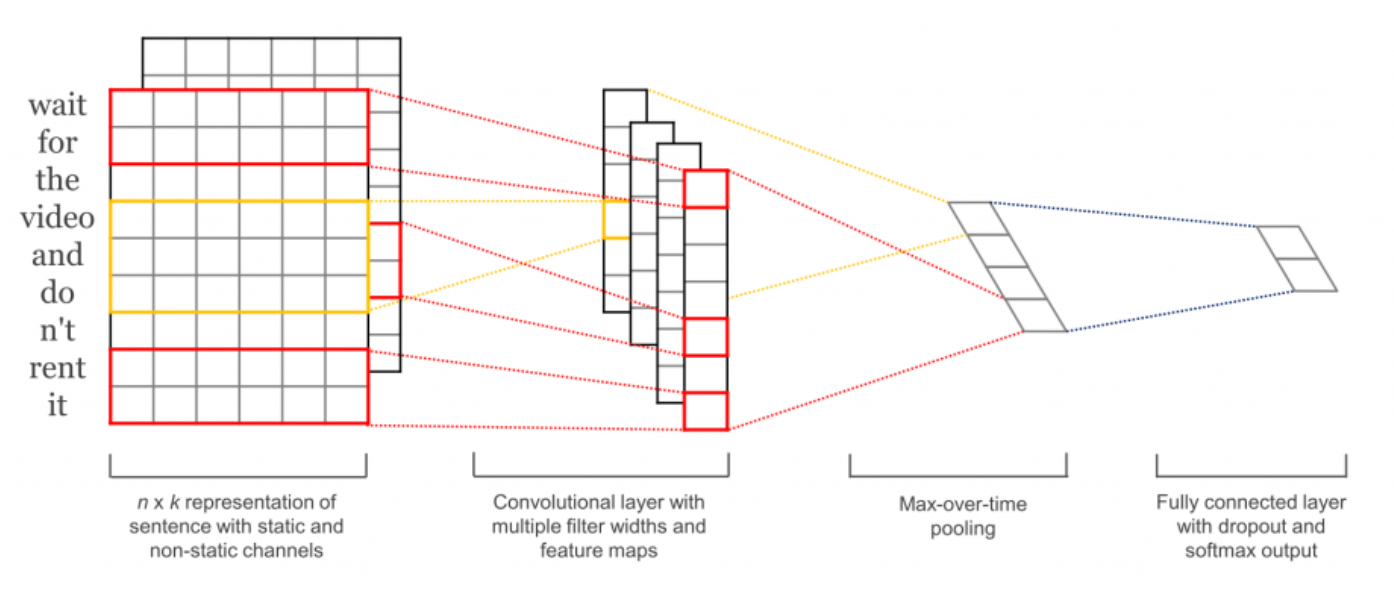
\includegraphics[width=0.6\textwidth]{1}
        \caption{CNN 模型框架图}
        \label{fig1}
    \end{figure}

    一个从第 $i$ 个单词开始包含 $h$ 个词的窗口可表示为:
    $$
    X_{i: (i + h - 1)} = (x_i, x_{i + 1}, \cdots, x_{i + h - 1})^T \in \mathbb{R}^{h \times k}
    $$

    我们定义一个 filter 为一个 $h \times k$ 的矩阵即:
    $$
    W \in \mathbb{R}^{h \times k}
    $$

    通过一个 filter 作用在一个词窗口上可以提取单个特征 $c_i$ 即:
    $$
    c_i = f(W \cdot X_{i: (i + h - 1)} + b)
    $$
    
    其中 $b \in \mathbb{R}$ 为偏差(Bias)项,$f$ 为激活函数如 ReLU, Sigmoid 等。

    我们定义卷积操作为,通过一个 filter 在一个句子上完整扫描一遍,得到一个特征图(Feature Map):
    $$
    \mathbf{c} = (c_1, c_2, \cdots, c_{n - h + 1})^T \in \mathbb{R}^{n - h + 1}
    $$

    再通过池化操作,对得到的 Feature Map 进行 Max Pooling 得到:
    $$
    \hat{c} = \max \mathbf{c}
    $$

    若最终有 $m$ 个 filter,则我们将得到:
    $$
    \mathbf{\hat{c}} = (\hat{c}_1, \hat{c}_2, \cdots, \hat{c}_m)^T \in \mathbb{R}^m
    $$

    最后通过对其进行一次线性变换即可得到最终的特征提取向量:
    $$
    \mathbf{y} = W_o \mathbf{\hat{c}} + \mathbf{b}_o
    $$

    其中 $W_o \in \mathbb{R}^{l \times m}, \mathbf{b}_o, \mathbf{y} \in \mathbb{R}^{l}$,$l$ 为情感标签种类。
    
    图 1 即展示了 CNN 模型的大致流程。

    \subsection{RNN 模型}

    \begin{figure}[h]
        \centering
        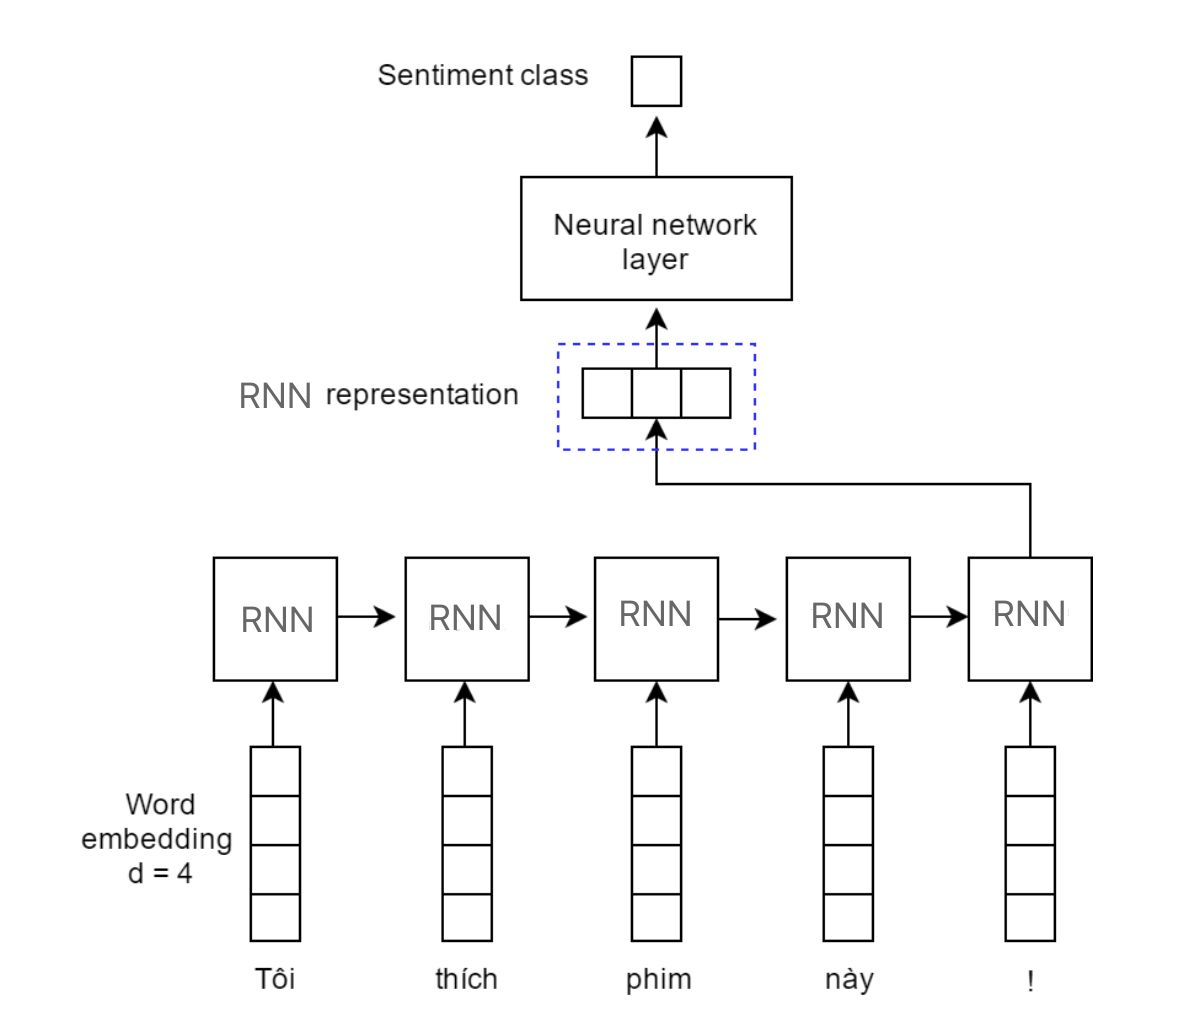
\includegraphics[width=0.6\textwidth]{2}
        \caption{RNN 模型框架图}
        \label{fig2}
    \end{figure}

    RNN 模型主要利用 RNN 结构,将句子中的词向量按照顺序作为 RNN 的输入,最终利用网络的输出($\mathrm{output} \in \mathbb{R}^{n \times h}$,$h$ 为 RNN 隐藏层大小)和隐藏层($\mathrm{hidden} \in \mathbb{R}^{h}$,默认只取最后一个隐藏层的隐藏状态),通过一些方式整合得到最终的特征提取向量:
    $$
    \mathbf{c} = f(\mathrm{output}, \mathrm{hidden}), \mathbf{y} = W_o \mathbf{c} + \mathbf{b}_o
    $$
    
    一种简易的方式为:
    $$
    f(\mathrm{output}, \mathrm{hidden}) = \mathrm{hidden}
    $$

    即直接利用隐藏层,忽略 $\mathrm{output}$,这种模型,在实验中我们将称其为朴素的 RNN 模型。

    另一种方式为利用 Attention 机制整合 $\mathrm{output}$ 与 $\mathrm{hidden}$,具体而言是:
    $$
    f(\mathrm{output}, \mathrm{hidden}) = \sum_{i = 1}^n \alpha_i \cdot \mathrm{output}_i
    $$

    其中系数 $\alpha_i$ 为:
    $$
    \alpha_i = \mathbf{v}^T \cdot \sigma(W_1 \cdot \mathrm{output}_i + W_2 \cdot \mathrm{hidden}) + b
    $$

    其中 $W_1, W_2 \in \mathbb{R}^{a \times h}, \mathbf{v} \in \mathbb{R}^a, b \in \mathbb{R}$ 均为模型参数,$\sigma$ 为 Sigmoid 激活函数,$a$ 为 Attention 层大小(超参数)。

    这种整合方式对应的模型,在实验中我们将称其为 RNN-Attention 模型。

    由于 RNN 网络本身包含朴素 RNN、LSTM、GRU 等多种,因此实验中也进行了区分。

    \subsection{baseline 模型}

    对于 baseline,主要实现了以下几种:

    \begin{itemize}
        \item \strong{MLP}:将每个词向量通过一层线性层和激活函数(取 ReLU),对每个句子做 Max Pooling,得到最终的隐藏向量,经过一层输出层得到最终的特征提取向量。
        \item \strong{Self-Attention}:将上述 RNN 模型中的 RNN 替换为若干个 Transformer Encoder 模块,即一层 Multihead Self-Attention 与一层 FFN 构成的残差网络。
        \item \strong{Self-Attention${}_{\pmb{p}}$}:在词向量输入 Encoder 之前,加上一个 Position Embedding 的偏置,以更好学习位置信息。
    \end{itemize}
    
    \newpage
    \section{实验结果与 baseline 对比}
    
    实验平台采用 PyTorch,随机种子均设置为 $1949$,使用了 V2 数据集。

    实验中统一设置词向量维度与隐藏层维度为 $64$,学习率为 $0.001$,L2 系数设置为 $10^{-6}$,Batch Size 为 $128$,优化器选择为 Adam,dropout 概率为 $0.5$,CNN 设置 $3, 4, 5$ 大小各 $100$ 个 filter,RNN layer 与 Transformer Encoder layer 数量均为 $2$,连续 $10$ 个 Epoch 验证集上表现不变好则停止训练(Early Stopping),至多进行 $200$ 个 Epoch。
    
    实验得到结果如下表:

    \begin{table}[H]
        \centering
        \begin{tabular}{cccc}
            \toprule
            \strong{模型} & \strong{Accuracy}($\%$) & \strong{Macro-averaging}($\%$) & \strong{Micro-averaging}($\%$) \\ \cline{1-4}
            \strong{CNN} & $\pmb{56.43}$ & $\pmb{55.84}$ & $\pmb{56.43}$ \\ \cline{1-4}
            \strong{RNN} & $27.72$ & $27.54$ & $27.72$ \\ \cline{1-4}
            \strong{LSTM} & $39.92$ & $39.84$ & $39.92$ \\ \cline{1-4}
            \strong{GRU} & $40.38$ & $40.57$ & $40.38$ \\ \cline{1-4}
            \strong{RNN-Atention} & $46.71$ & $46.47$ & $46.71$ \\ \cline{1-4}
            \strong{LSTM-Atention} & $48.73$ & $48.42$ & $48.73$ \\ \cline{1-4}
            \strong{GRU-Atention} & $48.47$ & $48.15$ & $48.47$ \\ \cline{1-4}
            \strong{MLP} & $52.12$ & $51.94$ & $52.12$ \\ \cline{1-4}
            \strong{Self-Attention} & $48.01$ & $48.36$ & $48.01$ \\ \cline{1-4}
            \strong{Self-Attention${}_{\pmb{p}}$} & $49.84$ & $50.00$ & $49.84$ \\
            \bottomrule
        \end{tabular}
        \caption{各模型及 baseline 表现}
	    \label{tab1}
    \end{table}

    可以看到,CNN 模型取得了最好的效果,其次是 MLP,而序列类型的模型都相对差一些。这一方面是因为数据集较小,序列类型模型对于数据集大小的要求较高,另一方面也可能表明不同类型网络,对于超参数的要求有一定区别。

    除此之外,也可以看到,在增加了 Attention 机制之后,RNN 模型的表现有了明显的提升,尽管仍然差于 MLP 与 CNN,但相对差距降低了许多。

    由于微平均与准确率差距较小,一般差别在小数点后 $5$ 位之后,因此表中数值均相同。

    \newpage
    \section{参数影响}

    下面为了得到更好的结果,我们仅探究各超参数对 CNN 以及 GRU-Attention 两个模型的影响。

    \begin{table}[H]
        \centering
        \begin{tabular}{cccc}
            \toprule
            \strong{参数} & \strong{Accuracy}($\%$) & \strong{Macro-averaging}($\%$) & \strong{Micro-averaging}($\%$) \\ \cline{1-4}
            \strong{default} & $48.47$ & $48.15$ & $48.47$ \\ \cline{1-4}
            $\pmb{k = h = a = 32}$ & $43.57$ & $43.54$ & $43.57$ \\ \cline{1-4}
            $\pmb{k = h = a = 128}$ & $50.49$ & $50.16$ & $50.49$ \\ \cline{1-4}
            $\pmb{k = h = a = 256}$ & $52.84$ & $52.33$ & $52.84$ \\ \cline{1-4}
            $\pmb{1}$ \strong{layer} & $51.92$ & $52.40$ & $51.92$ \\ \cline{1-4}
            $\pmb{3}$ \strong{layers} & $37.51$ & $37.16$ & $37.51$ \\ \cline{1-4}
            $\pmb{\mathrm{lr} = 10^{-1}}$ & $26.68$ & $23.16$ & $26.68$ \\ \cline{1-4}
            $\pmb{\mathrm{lr} = 10^{-2}}$ & $53.42$ & $52.88$ & $53.42$ \\ \cline{1-4}
            $\pmb{\mathrm{lr} = 10^{-4}}$ & $41.16$ & $41.07$ & $41.16$ \\
            \bottomrule
        \end{tabular}
        \caption{GRU-Attention 参数影响}
	    \label{tab2}
    \end{table}

    \begin{table}[H]
        \centering
        \begin{tabular}{cccc}
            \toprule
            \strong{参数} & \strong{Accuracy}($\%$) & \strong{Macro-averaging}($\%$) & \strong{Micro-averaging}($\%$) \\ \cline{1-4}
            \strong{default} & $56.43$ & $55.84$ & $56.43$ \\ \cline{1-4}
            $\pmb{k = h = a = 32}$ & $55.19$ & $54.57$ & $55.19$ \\ \cline{1-4}
            $\pmb{k = h = a = 128}$ & $57.21$ & $56.99$ & $57.21$ \\ \cline{1-4}
            $\pmb{k = h = a = 256}$ & $58.12$ & $57.63$ & $58.12$ \\ \cline{1-4}
            $\pmb{\mathrm{lr} = 10^{-1}}$ & $14.87$ & $9.87$ & $14.87$ \\ \cline{1-4}
            $\pmb{\mathrm{lr} = 10^{-2}}$ & $54.73$ & $54.32$ & $54.72$ \\ \cline{1-4}
            $\pmb{\mathrm{lr} = 10^{-4}}$ & $55.64$ & $55.36$ & $55.64$  \\
            \bottomrule
        \end{tabular}
        \caption{CNN 参数影响}
	    \label{tab3}
    \end{table}

    在隐藏层大小增大时,两个模型基本都能给出更高的准确率和 F1-Score,这是因为在一定范围内,隐藏层大小增加使得模型规模增大,加强了模型的拟合能力。

    而对 RNN,其中 layer 的数量增加却反而导致了性能的降低,这是由于过深的 RNN 网络可能会出现梯度传递出错、过拟合等问题。

    而在学习率上,都会出现,学习率过大,性能降低,而学习率过小,训练速度降低的问题,这也是从学习率本身定义上就可以解释的。

    可以看到,CNN 和 RNN 模型会在不同的参数设置下达到较好的效果,这也表明了不同模型具有特异性,统一的参数设置不一定完全公平。

    另一方面,在如学习率这样超参数的大致分析上,我们可以发现,大多数模型都会在一个较为接近的水平取得最优,而过大、过小都会极大程度上影响模型性能。因此对于这些超参数我们也可以通过实验和理论分析结合,来得到大致的经验法则。

    \newpage
    \section{思考与总结}

    \subsection{控制训练停止时间}

    实验中主要采用了 Early Stopping 与固定 Epoch 数结合,即设置一个最大的 Epoch 数量($200$),并在训练中,控制当连续若干次($10$ 次,每个 Epoch 一次)验证集上得出的准确率都相对于当前最优降低时,便提前停止训练。

    这种方式可以有效地防止模型出现明显的过拟合现象(由于验证集和测试集可认为来自统一分布),并且又能在一定程度上控制训练的最大时长。

    如果单纯控制迭代次数,将需要根据不同模型精细控制具体的迭代次数,将大大增加工作量;而若单纯使用 Early Stopping,又可能因为过于追求验证集上的表现,以及测试集的差异性出现一定过拟合。

    在这样的训练过程中,保存下测试集最好的模型数据作为 Checkpoint,最后用于测试集上指标测试,这样可以基本保证模型效果达到最好。

    \subsection{过拟合和欠拟合}

    对于过拟合,一方面可以使用 4.1 中提到的 Early Stopping 方法,另一方面也可以配合优化器(Adam, SGD, AdaGrad 等)的 L2、L1 正则化参数,用其控制模型的规模。

    同时通过增加 Dropout 层和 Normal 层,也可以降低模型复杂度,增强模型泛化程度,进而有助于防止过拟合。

    对于欠拟合,可考虑增大模型超参数,如本次实验中的 $h, k, a$ 等,或者加深网络结构,借此扩大模型的规模;也可以考虑引入更多的特征,比如一些任务中引入上下文特征。平台特征等。

    \subsection{梯度消失和梯度爆炸}

    两者主要发生的原因都是网络深度过深,导致反向求导过程中梯度值过小或过大,进而出现了参数难以更新(甚至神经元死亡)或者梯度误差过大等。

    典型的例子如 Sigmoid 激活函数求导结果过小,而初始参数往往较小,在较深网络时可能导致梯度趋向于 $0$;而在参数较大时,又可能导致梯度趋向于无穷。

    解决方案包括:
    \begin{itemize}
        \item 将 Sigmoid 激活函数改为 ReLU,有助于利用激活函数控制梯度的范围。
        \item 将 ReLU 激活函数改为 GeLU,PReLU,ELU,LeakyReLu 等,有助于防止结果均为负数导致的神经元死亡问题。
        \item 增加 BatchNormalization 层,更好的控制网络层与层之间的梯度转移。
        \item 将一些层改为残差网络结构,有助于减轻单层网络过度的影响,配合 Dropout 层也可更好的消除单个神经元的部分影响。
        \item 预训练加微调(Fine-Tuning),可以防止参数不合理初始化导致的部分问题,并且一定程度上可以加快训练速度。
    \end{itemize}

    \subsection{CNN, RNN, MLP 的比较}

    \begin{itemize}
        \item \strong{CNN}:
        \begin{itemize}
            \item \strong{优点}:
            \begin{enumerate}
                \item 卷积核共享,可以减少模型参数,一定程度上降低计算量,并增加模型泛化能力。
                \item 局部连接性,可以更好提取局部特征。
            \end{enumerate}
            \item \strong{缺点}:
            \begin{enumerate}
                \item 训练时,较容易收敛至局部最优。
                \item 池化操作容易丢失信息,忽略局部与整体的相关性。
            \end{enumerate}
            \item \strong{适用场景}:各种特征提取的任务,尤其是图像分类、图像检测、图像分割、关键点识别、图像生成等计算机视觉领域的相关任务。
        \end{itemize}
        \item \strong{RNN}:
        \begin{itemize}
            \item \strong{优点}:
            \begin{enumerate}
                \item 可以处理任意长度的输入、输出序列。
                \item 可以有效利用序列位置信息。
            \end{enumerate}
            \item \strong{缺点}:
            \begin{enumerate}
                \item 计算量较大,计算过程不能并行,导致训练效率较低。
                \item 容易出现梯度消失、梯度爆炸问题。
                \item 难以关注到序列中相隔较远的相关信息。
                \item 序列多向相关性效果较差。
            \end{enumerate}
            \item \strong{适用场景}:序列检测相关任务,尤其是文本翻译、图像描述、语义蕴涵、语音识别、文本摘要等自然语言处理领域的相关任务,但是在许多领域逐渐被 Transformers 取代。
        \end{itemize}
        \item \strong{MLP}:
        \begin{itemize}
            \item \strong{优点}:
            \begin{enumerate}
                \item 拟合能力极强,理论上可以拟合几乎任意连续函数。
                \item 在训练中,模型收敛速度较快。
                \item 方便并行处理与硬件加速。
            \end{enumerate}
            \item \strong{缺点}:
            \begin{enumerate}
                \item 容易收敛到局部最优。
                \item 容易出现过拟合问题。
                \item 隐藏层规模规律不明显,设计较困难。
                \item 难以利用输入的抽象结构信息。
            \end{enumerate}
            \item \strong{适用场景}:在各种模型的连接、整合输出等部分,常用到 MLP 来过滤;实际上通过一些 MLP 的设计,在特定情况下也可达到近似于别的网络类型的效果,比如 External-Attention 就与 Self-Attention 类似。
        \end{itemize}
    \end{itemize}

    \subsection{心得与体会}

    通过这次实验,我对于三种常用的深度学习神经网络结构都有了一定应用和理解,对于它们各自的优缺点、适用场景也有了自己的总结。

    感谢马老师和助教的悉心指导!

\end{document}
